% Chapter 3 - Results 

\chapter{Numerical experiments} % Main chapter title

\label{chap:results} % For referencing the chapter elsewhere, use \ref{Chapter1} 

\lhead{Chapter 3. \emph{Comparison of methods}} % This is for the header on each page - perhaps a shortened title

%----------------------------------------------------------------------------------------
\section{The main differences}
Using least squares will always give you a SPD system of equations which can be advantageous. However for second order equations this system is three times as big as if we were to solve it using more standard methods. Comparing the correctness of the solution as done in figure~\ref{fig:ConvergencePoisson} shows that the convergence rate is the same as for standard methods, but the value of the residual is slightly higher for the least squares method. This can be explained by the functional that is minimized. Notice that in the least squares methods you minimize the \textbf{square} of the residual, while with Galerkin you minimize the residual itself. Since the correctness of both methods are restricted by the smoothness of the solution and the number of discrete points LS-methods will minimize the residual squared down to a given precision and hence the residual itself to a slightly higher value. 
\newpage
\subsection{Poisson problem}
%
\begin{figure}[h!]
  \centering
  \begin{subfigure}[b]{0.48\textwidth}
	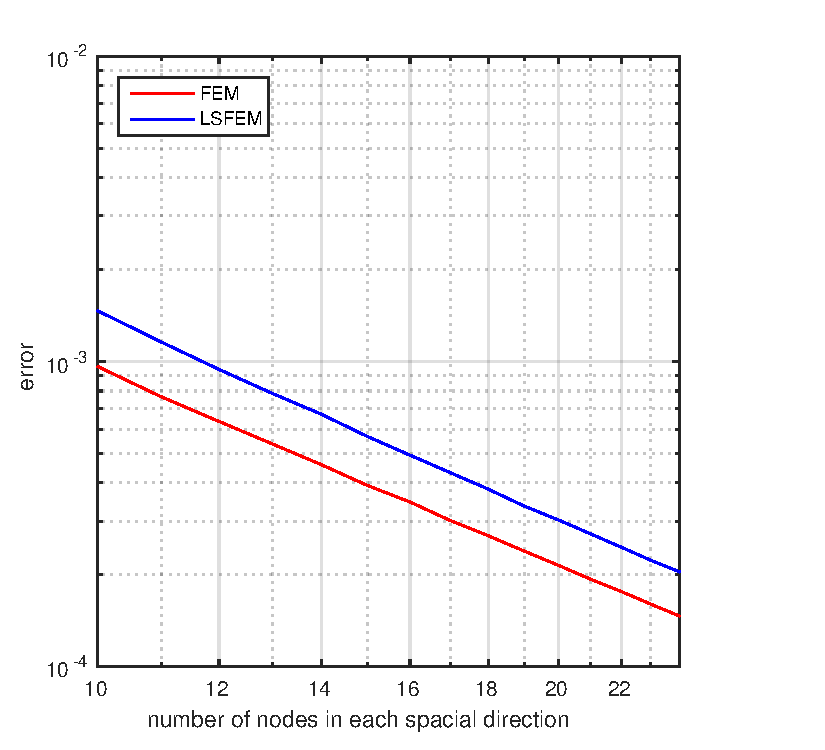
\includegraphics[width=\textwidth]{Figures/errorFEM-LSFEM.pdf}
  \end{subfigure}%
  \quad
  \begin{subfigure}[b]{0.48\textwidth}
	\includegraphics[width=\textwidth]{Figures/errorSpec-SpecLS.pdf}
  \end{subfigure}
          %(or a blank line to force the subfigure onto a new line)
  \vspace{-0.1\baselineskip}
  \caption{Convergence of Galerkin and corresponding least-squares formulation on the Poisson problem.}
  \label{fig:ConvergencePoisson}
\end{figure}
%
\begin{figure}[h!]
  \centering
  \begin{subfigure}[b]{0.48\textwidth}
	\includegraphics[width=\textwidth]{Figures/condFEM-LSFEM.pdf}
  \end{subfigure}%
  \quad
  \begin{subfigure}[b]{0.48\textwidth}
	\includegraphics[width=\textwidth]{Figures/condSpec-SpecLS.pdf}
  \end{subfigure}
          %(or a blank line to force the subfigure onto a new line)
  \vspace{-0.1\baselineskip}
  \caption{Condition number of Galerkin and corresponding least-squares formulation on the Poisson problem.}
  \label{fig:ConditionPoisson}
\end{figure}
%
\subsection{Diffusion transport equation convergence and condition number}
One of the disadvantages of least-squares methods is that the resulting
linear system is badly condition number. Now, let $\mathbf{b}$ be the vector field $[x,y]$, and let us see how the condition number scales with the parameters $\mu$ and $\beta$ in the equation 
\begin{align}
	-\mu \Delta u + \beta \mathbf{b} \cdot \nabla u = f
	\label{eq:difftransForConditionNumberPlotting}
\end{align}
%
\begin{figure}[h!]
  \centering
  \begin{subfigure}[b]{0.48\textwidth}
		\includegraphics[width=\textwidth]{Figures/Spec_difftrans_ConditionNumber.pdf}
  \end{subfigure}%
  \quad
  \begin{subfigure}[b]{0.48\textwidth}
		\includegraphics[width=\textwidth]{Figures/Spec-LS_difftrans_ConditionNumber.pdf}
  \end{subfigure}
          %(or a blank line to force the subfigure onto a new line)
  \vspace{-0.1\baselineskip}
	\caption{plot of the condition number when the parameters $\mu$ and $\beta$ are varied, $N=25,\mathbf{b} = -[x,y]$.}
  \label{fig:CondDifftransSpec}
\end{figure}
%
%
\begin{figure}[h!]
  \centering
  \begin{subfigure}[b]{0.48\textwidth}
		\includegraphics[width=\textwidth]{Figures/Spec_difftrans_Convergence.pdf}
  \end{subfigure}%
  \quad
  \begin{subfigure}[b]{0.48\textwidth}
		\includegraphics[width=\textwidth]{Figures/Spec_difftrans_Convergence_Neu.pdf}
  \end{subfigure}
          %(or a blank line to force the subfigure onto a new line)
  \vspace{-0.1\baselineskip}
	\caption{convergence plot with pure Dirichlet boundary conditions to the left and Neumann to the right  $\mathbf{b} = -[x,y]$.}
  \label{fig:ConvergenceDifftransSpec}
\end{figure}
%

\subsection{Diffusion transport equation surface plots}
\begin{figure}[h]
  \centering
  \begin{subfigure}[b]{0.48\textwidth}
	\includegraphics[width=\textwidth]{Figures/Spec_difftrans_aNeg.pdf}
  \end{subfigure}%
  \quad
  \begin{subfigure}[b]{0.48\textwidth}
	\includegraphics[width=\textwidth]{Figures/SpecLS_difftrans_aNeg.pdf}
  \end{subfigure}
          %(or a blank line to force the subfigure onto a new line)
  \vspace{-0.1\baselineskip}
	\caption{Surf plot of the numerical solution of the diffusion transport problem solved by Galerkin spectral methods to the left and least-squares to the right, $\mu = 10^{-4},N=25,\mathbf{b} = -[x,y]$.}
  \label{fig:SurfDiffTransPositive}
\end{figure}
%
\begin{figure}[h]
  \centering
  \begin{subfigure}[b]{0.48\textwidth}
	\includegraphics[width=\textwidth]{Figures/Spec_difftrans_aPos.pdf}
  \end{subfigure}%
  \quad
  %\begin{subfigure}[b]{0.48\textwidth}
	%\includegraphics[width=\textwidth]{Figures/SpecLS_difftrans_aPos.pdf}
  %\end{subfigure}
  \begin{subfigure}[b]{0.48\textwidth}
	\includegraphics[width=\textwidth]{Figures/SpecGLS_difftrans_aPos.pdf}
  \end{subfigure}
          %(or a blank line to force the subfigure onto a new line)
  \vspace{-0.1\baselineskip}
  \caption{Surf plot of the numerical solution obtained from spectral methods of the diffusion transport problem solved by Galerkin to the left and with a combined GLS method to the right, with smoothening factor $\delta = 0.05$, both plots use the same parameters $\mu = 10^{-4}, N=25,\mathbf{b} = [x,y]$.}
  \label{fig:SurfDiffTransPositive}
\end{figure}
%
%
\begin{figure}[h]
  \centering
  \begin{subfigure}[b]{0.48\textwidth}
	\includegraphics[width=\textwidth]{Figures/FEM_difftrans_aNeg.pdf}
  \end{subfigure}%
  \quad
  %\begin{subfigure}[b]{0.48\textwidth}
	%\includegraphics[width=\textwidth]{Figures/LSFEM_difftrans_aNeg.pdf}
  %\end{subfigure}
  \begin{subfigure}[b]{0.48\textwidth}
	\includegraphics[width=\textwidth]{Figures/GLSFEM_difftrans_aNeg.pdf}
  \end{subfigure}
          %(or a blank line to force the subfigure onto a new line)
  \vspace{-0.1\baselineskip}
	\caption{Surf plot of the numerical solution of the diffusion transport problem solved by Galerkin FEM to the left and the combined GLS method to the right, with smoothening factor $\delta = 0.05$, both plots use the same parameters, $\mu = 10^{-4},N=25,\mathbf{b} = -[x,y]$.}
  \label{fig:SurfDiffTransPositiveFEM}
\end{figure}

%
%\begin{figure}[h!]
  %\centering
  %\begin{subfigure}[b]{0.48\textwidth}
	%\includegraphics[width=\textwidth]{Figures/FEM_difftrans_aPos.pdf}
  %\end{subfigure}%
  %\quad
  %\begin{subfigure}[b]{0.48\textwidth}
	%\includegraphics[width=\textwidth]{Figures/LSFEM_difftrans_aPos.pdf}
  %\end{subfigure}
  %\begin{subfigure}[b]{0.48\textwidth}
	%\includegraphics[width=\textwidth]{Figures/GLSFEM_difftrans_aPos.pdf}
  %\end{subfigure}
          %%(or a blank line to force the subfigure onto a new line)
  %\vspace{-0.1\baselineskip}
  %\caption{Surf plot of the numerical solution of the diffusion transport problem solved by Galerkin FEM to the left ,least-squares to the right and the combined GLS method below with $\delta = 0.05$, all the plots use the same parameters $\mu = 10^{-4}, N=25,\mathbf{b} = [x,y]$.}
  %\label{fig:SurfDiffTransPositiveFEM}
%\end{figure}
%\begin{figure}[hl]
	%\centering
  %\includegraphics[width=80mm]{Figures/condFEM-LSFEM.pdf}
	%\caption{condition number of LSFEM and FEM}
	%\label{fig:conditionFEM}
%\end{figure}
%%
%%
%\begin{figure}[hl]
	%\centering
	%\includegraphics[width=80mm]{Figures/condSpec-SpecLS.pdf}
	%\caption{condition number of Spectral and LS-Spectral method}
	%\label{fig:conditionSpec}
%\end{figure}
%%

\subsection{Nonlinear results}

\begin{figure}[h]
  \centering
  \begin{subfigure}[b]{0.48\textwidth}
	\includegraphics[width=\textwidth]{Figures/Spec_Nonlin_Convergence_Jnum.pdf}
  \end{subfigure}%
  \quad
  \begin{subfigure}[b]{0.48\textwidth}
	\includegraphics[width=\textwidth]{Figures/Spec_Nonlin_Convergence.pdf}
  \end{subfigure}%
  \vspace{-0.1\baselineskip}
	\caption{Convergence plot of the numerical solution of the nonlinear diffusion transport equation solved by spectral methods, In the figure to the left a numerical jacobian has been calculated and in the figure to the right the analytical one is used. $\mu = 1,N=15,\mathbf{b} = -[x,y]$.}
  \label{fig:SurfDiffTransPositiveFEM}
\end{figure}
